\chapter{Introduction to normal mixture models}


%% it 2
\section{Definitions}

A good and thorough introductory book is the work of \cite{McL00} and
the reader is encouraged to study it to learn in depth about normal mixtures
and their clustering. 
We will here give a short overview of normal mixtures to fix notation and 
nomenclature.
The motivating idea behind mixture models is, that in real world examples
a sample might be suspected to arise from more than one population.
The original example of this, by Karl Pearson, who fitted two normal 
distributions with different means and variances.
In his paper Pearson analyzed measurements of forehead to body length of crabs
sampled from the bay of Naples. His mixture model-based approach suggested, 
that the crabs were evolving into two new subspecies.

here make clear we restrict to multivariate normal case.

Let $ \mu \in \mathbb{R}^p , \quad \Sigma \in \mathbb{R}^{p \times p} $ 
symmetric positive definite and $ \phi(- ; \mu, \Sigma) $ be the normal 
distribution with mean $ \mu $ and covariance matrix $ \Sigma $.


$ \pmb{Y}_1, \dots , \pmb{Y}_n $

\begin{definition}
    Suppose we have a random sample $ \pmb{Y}_1, \dots , \pmb{Y}_n $ with 
    probability density function $ \pmb{Y}_j \sim f(y_j) $ on 
    $\mathbb{R}^p$ We assume that the density $ f(y_j) $ of $ \pmb{Y}_j $ can 
    be written in the form 
    \[ f(y_j) = \sum_{k=1}^{K} \pi_k \phi_k (y_k; \mu, \Sigma) \]
    The $ \pi_k $ are called the component densities of the mixture and the 
    $\phi_k$ mixture components.
\end{definition}

here small note about restricted cases. give ref to 1.4??

\section{The EM-algorithm in sketch}

%% it 1
With this definition we immediately face the problem of how to fit these
mixture components to given data. A popular algorithm to solve this problem 
is the {\bf E}xpectation-{\bf M}aximization algorithm, abbreviated as 
EM-algorithm.

We give here a sketch of the EM-algorithm in the case of all normal mixture 
components, since it is the scope of this thesis and simplifies it 
considerably.

Suppose we have a $p-$dimensional dataset of $n$ samples $x_1, \dots ,x_n$,
onto which we would like to fit $K$ normal distributions 
$\phi_k,\ k \in {1,\dots , n}$. 
We introduce a further explaining variable $\pmb{Z}$ in 
$\textrm{Mat}^{n\times k}$, with entries in $[0,1]$ which represent the 
expectation that observation $i$ belongs to component $k$.

The EM-algorithm is a two step, iterative process consisting of an 'e'-step
and an 'm'-step.
% FIXME: inconsistent notation in Z and \tau
% FIXME: add remark about
In the e-step the expectation of component membership is updated.
\[ \tau_i(y_j;\Psi) = \phi_i(y_j;\mu_i, \Sigma_i)/ \sum_{k=1}^K \phi_k(y_j;
    \mu_k, \Sigma_k)\]
and in the m-step given the component membership information we update the 
component means and covariances by weighted versions of the usual estimators.
\[\mu_i = \sum_{j=1}^n \tau_{ij}y_j / \sum_{j=1}^n \tau_{ij}\]
\[\Sigma_i = \sum_{j=1}^n \tau_{ij} (y_j- \mu_i)(y_j-\mu_i)^\top / 
    \sum_{j=1}^n \tau_{ij}\]

here note about initialization methods.



\section{choice of notation}

% it 1
The classification of models in this paper relies heavily on the work of 
\cite{Cel95}, however, out of necessity for clarity, we break with their 
notation. 
So as to not confuse the reader we describe here in depth the differences in 
notation between \cite{Cel95} and ours.

The basis of classification in \cite{Cel95} is the decomposition of a
symmetric matrix into an orthogonal and a diagonal component.
A symmetric positive definite matrix $ \Sigma $ can be decomposed as follows
    \[ \Sigma = \lambda \pmb{D} \pmb{A} \pmb{D}^{\top} \]
with $ \pmb{D} $ an orthogonal matrix and $ \pmb{A} $ a diagonal matrix and
$ \lambda = \sqrt[\uproot{3}p]{det(\Sigma)} $ the $ p-th $ root of the 
determinant of $ \Sigma $.

This decomposition has an appealing geometric interpretation, with $ \pmb{D} $ 
as the \textit{orientation} of the distribution, $ \pmb{A} $ the \textit{shape},
and $ \lambda $ the \textit{volume}. The problem of notation comes from standard 
conventions in linear algebra, where the letters $A$ and $D$ are usually 
occupied by arbitrary and diagonal matrices respectively. Furthermore, we intend
to apply a variant of the Cholesky decomposition to $ \Sigma $, the 
$ \alpha\pmb{L}\pmb{D}\pmb{L}^{\top} $ decomposition. This obviously raises some
conflicts in notation.

Therefore we, from here on, when referring to the decomposition as described by 
\cite{Cel95}, will use the following modification of notation:

\begin{gather*} 
    \pmb{D} \longmapsto \pmb{Q} \\
    \pmb{A} \longmapsto \pmb{\Lambda} \\
    \lambda \longmapsto \alpha  \\
    \Sigma = \lambda \pmb{D} \pmb{A} \pmb{D}^\top =
        \alpha \pmb{Q} \pmb{\Lambda} \pmb{Q}^\top
\end{gather*}

These were chosen according to general conventions of linear algebra. $ \pmb{Q} $
is usually chosen for orthonormal matrices; $ \pmb{\Lambda} $ is often a choice 
for diagonal matrices eigenvectors and $ \alpha $ was somewhat arbitrarily 
chosen.


\section{Models of Covariance Matrices}

make clear that the models can not be translated one to one to ldlt model
% it 1
There is however an issue with the Cholesky decomposition. For 10 out of 14
cases as defined by \cite{Cel95}, there exists a canonical translation of
decompositions.
The 6 diagonal cases need no translation; the eigen and Cholesky decomposition
are equal to identity.
For the non-diagonal cases note that for a given sym. pos. def. matrix
$ \Sigma $ we have decompositions:
\[\Sigma = \alpha \pmb{Q \Lambda Q}^\top \quad \Sigma =\alpha \pmb{L D L}^\top\]
Since in both cases the bracketing matrices $ \pmb{Q} $ and $ \pmb{L} $ have 
determinant $ 1 $ the determinant of $ \Sigma $ falls entirely on $ \alpha $.
Therefore $ \alpha $, in these particular decompositions, is equal for both.
Celeux \& Grovaert vary $\Sigma$ by either varying or holding fixed the volume 
$(\alpha / \alpha_k)$, shape $(\pmb{\Lambda} / \pmb{\Lambda_k})$ and orientation
$(\pmb{Q} / \pmb{Q}_k)$.
These 3 times 2 cases would yield the 8 out of 14 cases of non-diagonal cases.
However there is no canonical transform for either variable orientation and 
fixed shape or fixed orientation and variable shape.
The reason for this is that in the $\pmb{LDL}^\top$ decomposition the lower
diagonal matrix $\pmb{L}$ holds some of the shape of the matrix, which in 
the eigendecomposition is in the $\pmb{\Lambda}$ matrix.
In fact, $\pmb{L}$ is orthogonal if and only if 
$\pmb{L} = \mathrm{Id}_{n\times n}$.
Therefore we can only decompose matrices where either both or neither shape and
orientation vary. See table \ref{table:param}.

While we could in theory construct the cases $\pmb{L}\pmb{D}_k\pmb{L}^\top$ and
$\pmb{L}_k \pmb{D} \pmb{L}^\top$, however they do not correspond to the desired
geometric intent behind the differentiation of models and are therefore not 
included.

make nice table(maybe sideways to account for parameter list)


\begin{table}[!htb]
    \centering
\rotatebox{90}
{
    \begin{tabular}{| c | c c c c c | c c c |}
        \hline
        Model & $\pmb{\Sigma}_k$ C\&G & volume & shape & orientation & parameters & $ \pmb{LDL}^\top $ & parameters & count \\
        \hline

        EII    & $ \alpha \pmb{I} $ & equal & equal & - & $ \alpha $ & same as C\&G & & 1 \\
        VII    & $ \alpha_k \pmb{I} $         & variable & equal & - & $ \alpha_k $ & & & $K$  \\
        EEI    & $ \alpha \pmb{\Lambda} $     & equal & equal & coordinate axes & $ \alpha, \lambda_i $ & & & $ 1+(p-1) $\\
        VEI    & $ \alpha_k \pmb{\Lambda} $ & variable & equal & coordinate axes & $ \alpha_k, \lambda_{i}$ & & & $ K+(p-1) $ \\
        EVI    & $ \alpha \pmb{\Lambda}_k $ &equal & variable & coordinate axes & $ \alpha, \lambda_{i,k} $ & & & $ 1+K(p-1) $ \\
        VVI    & $ \alpha_k \pmb{\Lambda}_k $ & variable & variable & coordinate axes & $ \alpha_k, \lambda_{i,k} $ & & & $ K+K(p-1) $ \\
        \hline
        EEE    & $ \alpha \pmb{Q \Lambda Q}^\top $ &equal & equal & equal & $ \alpha, \lambda_{i}, q_{i,j} $ & $ \alpha \pmb{LDL}^{\top} $ & $ \lambda , d_i, l_{i,j} $ & $ 1+(p-1)+\frac{p(p-1)}{2} $ \\
        \hline
        EVE    & $ \alpha \pmb{Q \Lambda}_k \pmb{Q}^\top $ &equal & variable & equal & $ \alpha, \lambda_{i,k}, q_{i,j} $  & doesn't exist & & $ 1+K(p-1)+\frac{p(p-1)}{2} $ \\
        \hline
        VEE    & $ \alpha_k \pmb{Q \Lambda Q}^\top $ & variable & equal & equal & $ \alpha_k, \lambda_{i}, q_{i,j} $ & $ \alpha_k \pmb{LDL}^\top $ & $ \lambda_k , d_i, l_{i,j} $ & $ K+p+p^2\frac{p(p-1)}{2} $ \\
        \hline
        VVE    & $ \alpha_k \pmb{Q \Lambda}_k \pmb{Q}^\top $ &variable & variable & equal & $ \alpha_k, \lambda_{i,k}, q_{i,j} $ & & & $ K+K(p-1)+\frac{p(p-1)}{2} $ \\
        EEV    & $ \alpha \pmb{Q}_k \pmb{\Lambda} \pmb{Q}_k^\top $ &equal & equal & variable & $ \alpha, \lambda_{i}, q_{i,j,k} $ &  don't exist  & & $ 1+(p-1)+K\frac{p(p-1)}{2} $ \\
        VEV    & $ \alpha_k \pmb{Q}_k \pmb{\Lambda} \pmb{Q}_k^\top $ &variable & equal & variable & $ \alpha_k, \lambda_{i}, q_{i,j,k} $ & & & $ K+(p-1)+K\frac{p(p-1)}{2} $ \\
        \hline
        EVV    & $ \alpha \pmb{Q}_k \pmb{\Lambda}_k \pmb{Q}_k^\top $ & equal & variable & variable & $ \alpha, \lambda_{i}, q_{i,j,k} $ & $ \alpha \pmb{L}_k \pmb{D}_k \pmb{L}_k^\top $ & $ \lambda, d_{i,k}, l_{i,j,k}\ j>i $ & $ 1+pK+K\frac{p(p-1)}{2} $  \\
        VVV    & $ \alpha_k \pmb{Q}_k \pmb{\Lambda}_k \pmb{Q}_k^\top $ & variable & variable & variable & $ \alpha_k, \lambda_{i}, q_{i,j,k} $ & $ \alpha_k \pmb{L}_k \pmb{D}_k \pmb{L}_k^\top $ & $ \lambda_k, d_{i,k}, l_{i,j,k}\ j>i $ & $ K+pK+K\frac{p(p-1)}{2} $ \\
        \hline
    \end{tabular}

}

\caption{Table of Parameters}
\label{table:param}
\end{table}

\clearpage


\section{problems of EM}


The EM-algorithm has stalling problems especially close to a local optimum.
% it 1
In their seminal work, \cite{Dem77}, have proven that the EM-algorithm 
converges under mild regularity conditions. 
%TODO: talk more about Dem77, in more detail about convergence conditions
However, convergence does not guarantee fast convergence. In fact, a lot of 
the work, that has gone into the research around the EM-algorithm has been 
concerned with speeding up convergence, see \cite{McL00}[section 2.17].
In common software implementations, %TODO: mostly initial clustering?? not sure
The concern here is that a slowing in convergence might be mistaken for actual
convergence.

% it 1
This phenomenon is not infrequent and in difficult mixtures quite visible.
To illustrate let us look at a particular mixture taken from \cite{Mar92} and
the {\tt nor1mix} package from CRAN.

\begin{Schunk}
\begin{Sinput}
> library("nor1mix")
> MW.nm9 ## Trimodal mixture
\end{Sinput}
\begin{Soutput}
'Normal Mixture' object 	 ``#9 Trimodal'' 
       mu sigma    w
[1,] -1.2  0.60 0.45
[2,]  1.2  0.60 0.45
[3,]  0.0  0.25 0.10
\end{Soutput}
\end{Schunk}


show an example using nor1mix



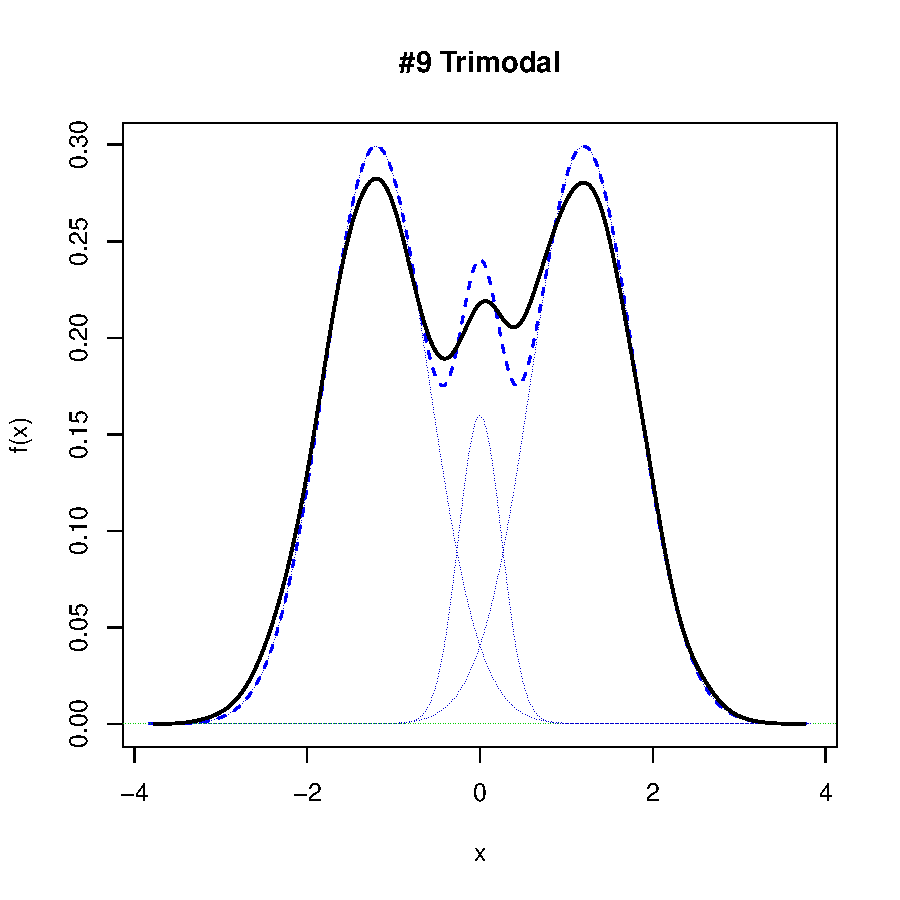
\includegraphics{chapter1-003}



then an illustration of MW examples of pathological cases


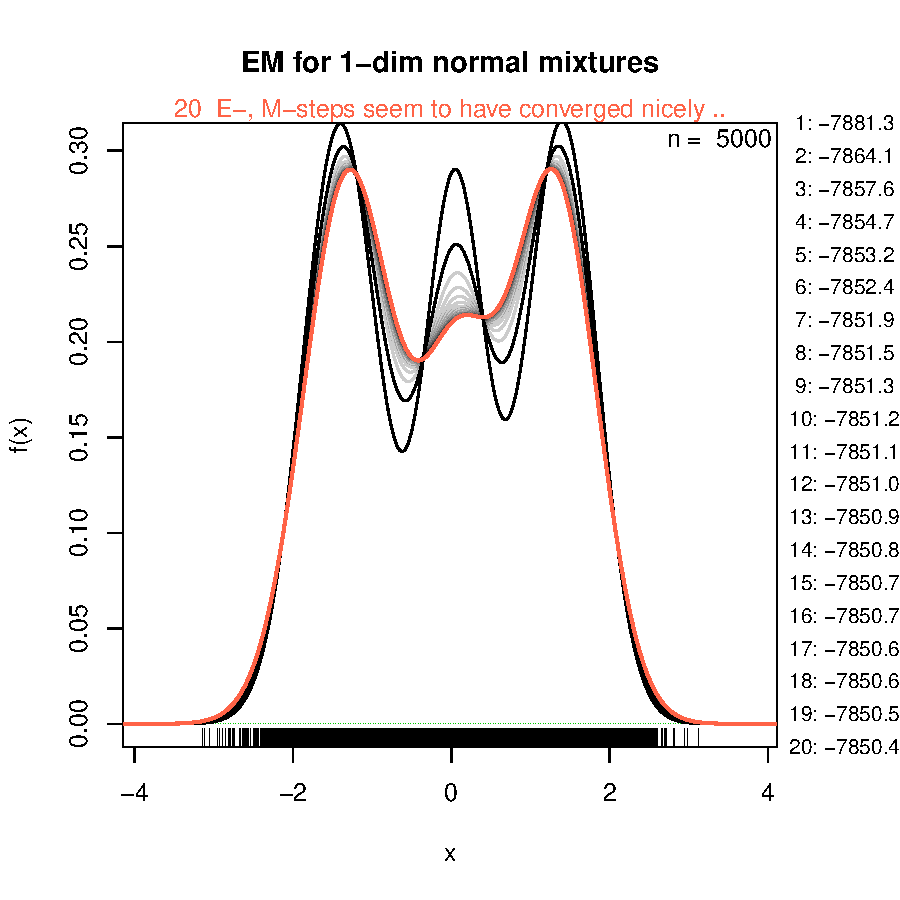
\includegraphics{chapter1-nor1mixEx}


%yay, got figure to print. solution was use of fig=TRUE, instead of various mutations like figure=true.

here we see how change in loglik seems to stagnate. However, this does not stay that way, if we let EM run a bit further.


\begin{figure}
\begin{center}
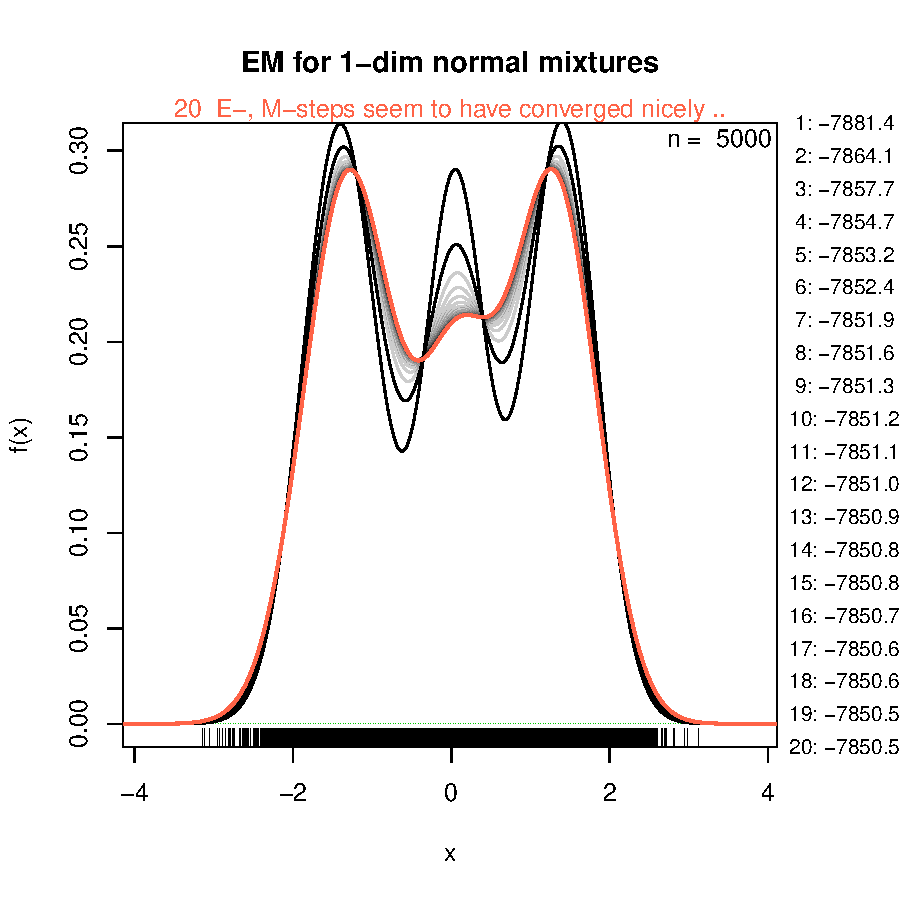
\includegraphics{chapter1-006}
\end{center}
\caption{200 EM steps}
\label{adfafdafds}
\end{figure}

to conclude example show part of mixest that shows it takes 1200 iterations to converge

In fact, it seems that the previous solution is a saddle point in the likelihood function, where EM has chronic problems continuing improvements.

give 2D demonstration.

maybe show Marr Wand's examples of 'difficult' mixtures

give conclusion recapping the just demonstrated, and lead in for next chapter




%%%%%%%%%%%%%%%%%%%%%%%%%%%%%%%%%%%%%%%%%%%%%%%%%%%%%%%%%%%%%%%%%%%%%%%%%%%%%%%%

\chapter{The {\tt norMmix} Package}

% it 1
For this thesis, an R package was developed that implements the algorithm
that fits multivariate normal mixtures to given data.
There is a lot of unused code still in the package. These were at one point
implemented used and discarded. They are still included for demonstration.
The norMmix package is constructed around the {\tt norMmix} object, that 
codifies a {\tt nor}mal {\tt M}ultivariate {\tt mix}ture model,  and the {\tt 
llnorMmix()} function, that calculates the log-likelihood given a model and 
data.


% it 1
The package contains the following functionality:
\begin{description}
    \item [{\tt norMmix}] {\tt norMmix()} is the 'init-method' for 
        {\tt norMmix} objects. There exist {\tt is.norMmix} {\tt rnorMmix} and
        {\tt dnorMmix} functions.
    \item [parametrization] The main functions that handle reparametrization
        of models from and to $\pmb{LDL}^\top$ decomposition are {\tt nMm2par}
        and {\tt par2nMm}, which are inverse to each other.
    \item [MLE] The function {\tt norMmixMLE} marries the main components of 
        this package. It initializes a model and parametrizes it for use with 
        {\tt optim}
    \item [fitting] Using {\tt norMmixMLE}, the function fitnMm allows fitting 
        of multiple models and components. Functions analyzing the output of 
        this are also provided, e.g. {\tt BIC} and {\tt pring} methods.
    \item [misc] There are also various methods of generics, like {\tt logLik,
        print, BIC, AIC} and {\tt nobs} as well as various {\tt print} methods.
    \item [example objects] Following the paper of \cite{Mar92} various example
        objects are provided and used for study. They follow the naming 
        convention: MW + dimension + number. for example {\tt MW213} for the 
        13th model of dimension 2.
\end{description}

relies on {\tt optim()} generic optimizer. maximizes llnormix by varying model 
parameters.

since mclust is one of the more popular packages implementing the EM algo, we 
employ a lot of functions from mclust, to keep things around EM as similar as 
possible.

% it 1
Conceptually, at the start of a fitting algo, e.g. EM we need to initialize a
mixture object. % TODO we (will?) have translation methods to and from mclust
thereafter the paths diverge. at the heart of norMmix's functionality
lie the functions: llnorMmix and nMm2par which are in turn employed by 
norMmixMLE to funnel a mixture object into optim and give optim a function
to optimize.

also relies on {\tt mixtools} package for random generating function 
{\tt rnorMmix} using {\tt rmvnorm}.

\section{finer details of {\tt norMmix} package}

about Cholesky decomp as ldlt. has advantages: fast, parametrically 
parsimonious, can easily compute loglikelihood

%it 1

maybe reread section in McLachlan about accelerating EM algo

not possible to sensibly compare normal mixtures except maybe a strange sorting 
algorithm using mahalanobis distance or Kullback-Leibler distance or similar
(Hellinger), but not numerically sensible to integrate over potentially 
high-dimensional spaces.

So comparison of algos done through throwing difficult mixtures and 
non-mixtures at it and hoping that norMmix finds better solutions than EM. So
the criteria for "better fit" are 1. better log-likelihood 2. correct model, 
where EM fails.




%%%%%%%%%%%%%%%%%%%%%%%%%%%%%%%%%%%%%%%%%%%%%%%%%%%%%%%%%%%%%%%%%%%%%%%%%%%%%%%%

\chapter{Comparing Algorithms}

\section{On The Development of {\tt norMmix}}

general list of (not necessarily mathematical) dead-ends in the development 
life of the norMmix package.
argue why this is in this section?? because, as a BScT, the learning is as much
part of the research as the results.

here on why logit doesnt work

% it 1
One dead-end was the parametrization of the weights of a mixture using the 
{\tt logit} function.

\begin{Schunk}
\begin{Sinput}
> logit <- function(e) {
+     stopifnot(is.numeric(e) ,all(e >= 0), all.equal(sum(e),1))
+     qlogis(e[-1L])
+ }
> logitinv <- function(e) {
+     if (length(e)==0) {return(c(1))}
+     stopifnot(is.numeric(e))
+     e<- plogis(e)
+     sp. <- sum(e)
+     w <- c((1-sp.), e)
+ }
\end{Sinput}
\end{Schunk}

This uses the logistical function {\tt logis} to transform to reduce the number
of weights from $K$ to $K-1$. Much like {\tt clr1}, given a list of weights 
{\tt logit} will transform them and {\tt logitinv} will correctly reverse the 
transformation. However, unlike {\tt clr1}, it will not transform an arbitrary 
list of length $K-1$ into a valid weight parameter. For example:

\begin{Schunk}
\begin{Sinput}
> w <- runif(7); ret <- logitinv(w)
> ret
\end{Sinput}
\begin{Soutput}
[1] -3.3177307  0.6364078  0.6511485  0.6018082  0.6783043  0.5517875  0.6631182
[8]  0.5351562
\end{Soutput}
\end{Schunk}

The issue here is that the last line of {\tt logitinv}, which is necessary to 
sum to one, but results in a negative value in {\tt ret[1]} which is not a 
valid weight. The underlying issue is that not every tuple in $\R^{K-1}$ is 
a result of {\tt logit}.

The option to use {\tt logit} is still an argument to {\tt norMmixMLE} by 
specifying {\tt trafo="logit"}, but it shouldn't be used.

on forcePositive and previous m-step, lead to decision to use mclust msteps.

% it 1
Another issue during development cropped up during fitting of high dimensional
data. We studied the dataset {\tt SMI.12} from the package {\tt copula}:

\begin{Schunk}
\begin{Sinput}
> data(SMI.12, package="copula")
> str(SMI.12)
\end{Sinput}
\begin{Soutput}
 num [1:141, 1:20] 16.1 15.7 15.7 16.1 16.6 ...
 - attr(*, "dimnames")=List of 2
  ..$ : chr [1:141] "2011-09-09" "2011-09-12" "2011-09-13" "2011-09-14" ...
  ..$ : chr [1:20] "ABBN" "ATLN" "ADEN" "CSGN" ...
\end{Soutput}
\end{Schunk}

A consequence of high dimensions is that matrix multiplication is no longer
very stable. As a result, the covariance matrices produced by our own 
implementation of the EM-algorithms m-step ({\tt mstep.nMm}) were not positive
definite.
In the case of {\tt SMI.12}, several covariance matrices are degenerate, which
results in cancellation error with near-zero entries.
We attempted to correct this with the function {\tt forcePositive}, which 
simply tries to set $\pmb{D}$ in $\pmb{LDL}^\top$ greater than zero.
This didn't resolve the issue, since a non-negligible part of the numerical
error was in the $\pmb{L}$ matrix and the resultant covariance matrix was still
not positive definite.

We eventually resolved this issue by abandoning our own implementation and 
using the functions from the {\tt Mclust} package. Not only were these 
numerically stable they were also able to differentiate between models, whereas
ours would assume VVV for every fit.

testing of mvtnorm as proof that ldlt is in fact faster parametrization

mention, that there may be faster ways to apply backsolve. 
quote knuth about premature optimization.

\section{General Setup}
display abilities of norMmix on its own. can find correct models

Mention, that mclust doesn't depend on seed(double check) and therefore norMmix has 
advantage of 'confidence intervals'. We can run 50 simulations and see if there
might be more sensible clusters.

maybe apply to MW[0-9] objects?

not sure

as in Raftery2002, Benaglia2009, Roeder 1997, maybe compare to MISE of various 
forms. They all did and see it as adequate method for comparing accuracy of 
algorithm.

also wanted is accuracy of model selection. generate from model and then compare
fitted to original. either by acc-model==fit-model and acc-k==fit-k or acc-ll - fit-ll.

\section{Findings}

%%%%%%%%%%%%%%%%%%%%%%%%%%%%%%%%%%%%%%%%%%%%%%%%%%%%%%%%%%%%%%%%%%%%%%%%%%%%%%%%

\chapter{Discussion}

